\documentclass[conference]{IEEEtran}
\IEEEoverridecommandlockouts
\usepackage[utf8]{inputenc}
\usepackage[T1]{fontenc}
\usepackage[english]{babel}
\usepackage{newtxtext, newtxmath} 
\usepackage{graphicx}          
\usepackage{float}             
\usepackage{amsmath}  
\usepackage{booktabs}         
\usepackage[font=small]{caption}
\usepackage{subcaption}
\usepackage[acronym]{glossaries}
\newacronym{bcet}{BCET}{Balance Contrast Enhancement Technique}
\newacronym{csf}{CSF}{Cerebrospinal Fluid}
\newacronym{fcm}{FCM}{Fuzzy C-Means}
\newacronym{flair}{FLAIR}{Fluid-Attenuated Inversion Recovery}
\newacronym{fn}{FN}{False Negative}
\newacronym{fom}{FOM}{Figure of Merit}
\newacronym{fp}{FP}{False Positive}
\newacronym{mri}{MRI}{Magnetic Resonance Imaging}
\newacronym{msd}{MSD}{Medical Segmentation Decathlon}
\newacronym{roi}{ROI}{Region of Interest}
\newacronym{tn}{TN}{True Negative}
\newacronym{tp}{TP}{True Positive}
\usepackage[colorlinks=true, linkcolor=blue, citecolor=blue, urlcolor=blue]{hyperref}
\begin{document}
\title{Robust Edge Detection in MRI Glioblastomas: Validating and Optimizing the Zotin Pipeline}
\author{
    \IEEEauthorblockN{Alessandro Sartori}
    \IEEEauthorblockA{\textit{Department of Electrical and Information Engineering (DEI)} \\
    \textit{Polytechnic University of Bari}\\
    Bari, Italy \\
    a.sartori@studenti.poliba.it}
}
\maketitle 
\begin{abstract}
Correctly identifying the edges of glioblastomas on \gls{mri} is important for planning surgery. This work reproduces and then optimizes the unsupervised edge detection pipeline of Zotin et al. (2018) \cite{zotin2018edge}, based on \gls{bcet} and Fuzzy C-Means clustering. Tests on 484 patients show that the baseline pipeline looks visually reasonable but performs poorly on clinical metrics, with mean Sensitivity of just 10.7\%. To address this, the proposed pipeline adds dynamic volumetric slice selection and switches to \gls{flair} sequences to reduce cerebrospinal fluid artifacts. This raises mean Sensitivity by 132\% and mean \gls{fom} by 46\%, suggesting that the input modality and slice choice matter as much as the segmentation algorithm itself.
\end{abstract}
\begin{IEEEkeywords}
Edge Detection, MRI, Glioblastoma, Fuzzy C-Means, FLAIR, Optimization.
\end{IEEEkeywords}
\section{Introduction}\label{sec:intro}
Extracting brain tumor boundaries from \gls{mri} accurately is an important task in medical image analysis, since it affects how surgery is planned and how nearby tissue is evaluated. Zotin et al. proposed an automated pipeline for this problem \cite{zotin2018edge}, organized into three phases. First, an image enhancement stage uses a median filter for noise suppression and \gls{bcet} to improve contrast in the region of interest. Second, a segmentation stage applies \gls{fcm} clustering to divide the image into homogeneous classes by pixel intensity, followed by the Canny operator to extract thin edges of the tumor. Finally, a data-analysis stage evaluates the result with metrics such as \gls{fom}, Sensitivity, and Accuracy, comparing the predicted edges to reference maps drawn by human experts \cite{pratt1979quantitative}. The original study reports good results on a small, hand-picked set of images, but unsupervised intensity-based methods do not necessarily generalize to the larger anatomical variability found in clinical datasets. This motivates further pre-processing, such as morphological skull-stripping \cite{hooda2014brain} and deterministic centroid initialization for \gls{fcm} \cite{benson2016brain, szilagyi2003mri}. The rest of this paper is organized as follows. Section \ref{sec:baseline} reproduces the baseline pipeline as closely as possible to the original paper and validates it on a much larger dataset, showing where it struggles. Section \ref{sec:optimized} proposes an optimized pipeline that addresses these issues through dynamic slice selection, a switch to \gls{flair} sequences, and a more tolerant evaluation metric. Section \ref{sec:comparison} compares the baseline and optimized results and discusses the role of \gls{csf} interference. Section \ref{sec:conclusions} summarizes the findings.
\section{Theoretical Background}\label{sec:background}
This section describes the image processing techniques used for tumor edge detection, following the methodology of Zotin et al. \cite{zotin2018edge}. The pipeline has three phases: pre-processing for noise reduction and contrast enhancement, clustering-based segmentation, and edge extraction. \gls{mri} scans are affected by noise and artifacts coming from the physical limits of the acquisition equipment. The methodology uses a Median Filter, a non-linear rank-order filter, to suppress impulse noise while preserving edge sharpness. Given a kernel $K$ centered at $(x,y)$, the operation is defined as

\begin{equation}
    I_{new}(x,y) = \text{med}_{(k_x,k_y) \in K} \{ I_{old}(k_x,k_y) \}
\end{equation}
To further highlight \glspl{roi}, the \gls{bcet} is applied. This technique expands the image contrast without altering the histogram pattern \cite{zotin2018edge} using a parabolic function
\begin{equation}
    I_{new} = a(I_{old} - b)^2 + c
\end{equation}
where coefficients are computed deterministically based on the maximum and minimum intensity values of the output image ($I_{new}$), and the mean value of intensity of the output image ($E$)
\begin{equation}
b = \frac{h^2(E - L) - s(H - L) + l^2(H - E)}
{2[h(E - L) - e(H - L) + l(H - E)]}
\end{equation}
\begin{equation}
a = \frac{H - L}{(h - l)(h + l - 2b)}
\end{equation}
\begin{equation}
c = L - a(l - b)^2
\end{equation}
\begin{equation}
s = 1/N \sum_{i=1}^{N}I_{old}^2(i)
\end{equation}
Segmentation aims to partition image pixels into distinct segments based on similarity. Unlike "hard" clustering, \gls{fcm} \cite{bezdek1981pattern} is a "soft" method that assigns a membership degree $u_{ik} \in [0,1]$ to each pixel. The algorithm iteratively minimizes the objective function
\begin{equation}
    F(W,V) = \sum_{i=1}^{c} \sum_{k=1}^{n} (u_{ik})^m \cdot ||x_k - v_i||^2
\end{equation}
where $ 1\le m \le \infty$ is the "fuzziness" index, $w_{ik}\in [0,1]$ is the degree of membership of $ x_k$ in the $i$th cluster, and $\|x_k - v_i\|^2$ represents the distance between the data $x_k$ and the cluster center $v_i$. This soft assignment is well suited to the Partial Volume Effect inherent to \gls{mri}: a single voxel at the boundary between two tissue types can physically contain a mixture of both, so a hard partition such as $k$-means is forced to assign it entirely to one class, while \gls{fcm}'s fractional membership reflects this underlying ambiguity directly, generally producing more anatomically coherent clusters at tissue boundaries. A simpler alternative, Otsu's global thresholding, is computationally cheaper and depends on a single, easily interpreted parameter, but it requires a histogram with well-separated bimodal peaks; \gls{mri} histograms are frequently smoothed by noise and tissue heterogeneity, in which case Otsu's single rigid boundary misclassifies voxels that \gls{fcm}'s gradual membership transition handles more robustly. Finally, an edge is a strong local change in brightness that usually corresponds to an anatomical boundary. The Canny algorithm is used here because it satisfies three criteria identified by Pratt \cite{pratt1979quantitative}: low error rate, precise localization, and a single-pixel response. The process has four stages:
\begin{enumerate}
    \item \textbf{Smoothing}: Convolution with a Gaussian filter to eliminate residual noise.
    \item \textbf{Gradient Calculation}: Determination of spatial gradient magnitude and direction.
    \item \textbf{Non-Maximal Suppression}: Thinning the gradient ridges to isolate the pixels with the highest intensity change.
    \item \textbf{Hysteresis Thresholding}: Validating edges using high and low thresholds to differentiate true anatomical boundaries from noise-induced segments.
\end{enumerate}
\section{Baseline Methodology and Experimental Validation}\label{sec:baseline}
To quantitatively validate the predicted edge maps against the expert-annotated boundaries, the data-analysis phase of Zotin et al. \cite{zotin2018edge} is formalized using the confusion-matrix quantities \gls{tp}, \gls{tn}, \gls{fp}, \gls{fn} (denoted $\mathrm{TP}$, $\mathrm{TN}$, $\mathrm{FP}$, $\mathrm{FN}$ from here on), and the reference edge count $\mathrm{RECnt}=\mathrm{TP}+\mathrm{FN}$. The percentage of correctly detected pixels ($\mathrm{Pcd}$), the percentage of non-detected pixels ($\mathrm{Pnd}$), the percentage of false alarms ($\mathrm{Pfa}$), Sensitivity, Accuracy, and the \gls{fom} \cite{pratt1979quantitative} are computed as
\begin{equation}
\mathrm{Pcd} = \mathrm{Sensitivity} = \frac{\mathrm{TP}}{\mathrm{RECnt}}\\[0.5em] \quad
\end{equation}
\begin{equation}
	\mathrm{Pnd} = \frac{\mathrm{FN}}{\mathrm{RECnt}}\\[0.5em] \quad
\end{equation}
\begin{equation}
	\mathrm{Pfa} = \frac{\mathrm{FP}}{\mathrm{RECnt}}\\[0.5em] \quad
\end{equation}
\begin{equation}
	\mathrm{Accuracy} = \frac{\mathrm{TP}+\mathrm{TN}}{\mathrm{TP}+\mathrm{TN}+\mathrm{FP}+\mathrm{FN}}
	\\[0.5em] \quad
\end{equation}
\begin{equation}
	\mathrm{FOM} = \frac{1}{\max(\mathrm{RECnt},\mathrm{AECnt})}\sum_{i=1}^{\mathrm{AECnt}} \frac{1}{1+\alpha d_i^2}
\end{equation}

where $\mathrm{AECnt}$ is the number of detected edge pixels, $d_i$ is the distance of the $i$-th detected pixel to its nearest reference edge pixel, and $\alpha=1/9$ is Pratt's empirically calibrated constant \cite{pratt1979quantitative}. Since $\mathrm{Pcd}$ and Sensitivity share the same definition, they are numerically identical and are reported interchangeably. The baseline pipeline is a strict reproduction of \cite{zotin2018edge}, but it is validated on a scale two orders of magnitude larger than the original study: 484 multiparametric volumes (T1, T1Gd, T2, \gls{flair}, with expert-annotated masks) from the Brain Tumor task of the \gls{msd} \cite{antonelli2022medical}, against the 30 hand-picked images used by Zotin et al. For each patient, the T2 channel is extracted and a single fixed axial slice at the volumetric midpoint is processed, mirroring the 2-D, per-image nature of the original study. Two additions, left unspecified by \cite{zotin2018edge}, were required to make the pipeline operate on this dataset. In the baseline (and also for the optimized pipeline next in \ref{sec:optimized}), predicted edges are highlighted in red, expert ground truth in green, and their combined overlay -if they match- in yellow, for the best, median, and worst \gls{fom} cases over the 484 BRATS patients. First, unlike the pre-cropped images used in the original work, \gls{msd} volumes contain a large all-zero background outside the skull; a robust brain mask, obtained via Otsu thresholding followed by hole-filling and largest-component extraction, restricts both the \gls{bcet} statistics and the \gls{fcm} clustering to intracranial tissue. Second, since \cite{zotin2018edge} neither specifies the number of clusters $c$ nor a rule for selecting the tumor cluster once \gls{fcm} has converged, $c$ is fixed at 4, consistent with Gonzalez and Woods' treatment of clustering-based segmentation, where the number of clusters is specified directly rather than estimated automatically. The tumor candidate is then selected among the brightest clusters by scoring the solidity times the area of their largest connected component, excluding any cluster occupying more than 40\% of the brain mask, since the normal brain-tissue cluster is itself large and solid and would otherwise be mistaken for the lesion. Figure \ref{fig:baseline_pipeline} shows every stage of this pipeline applied to a single patient. Panel (\ref{fig:baseline_input}) shows the input T2 slice alongside the radiologist's annotation; panel (\ref{fig:baseline_preprocessing}) shows the result of median filtering, Otsu brain masking, and BCET enhancement; panel (\ref{fig:baseline_segmentation}) shows the four-class FCM segmentation and the isolated tumor candidate; panel (\ref{fig:baseline_edge_extraction}) shows the morphological boundary extracted from this candidate, overlaid on the original slice; and panel (\ref{fig:baseline_validation}) compares this predicted boundary against the expert ground truth.
\begin{figure}[htbp]
    \centering
    \captionsetup[subfigure]{justification=centering} 
    \begin{subfigure}[b]{\columnwidth}
        \centering
        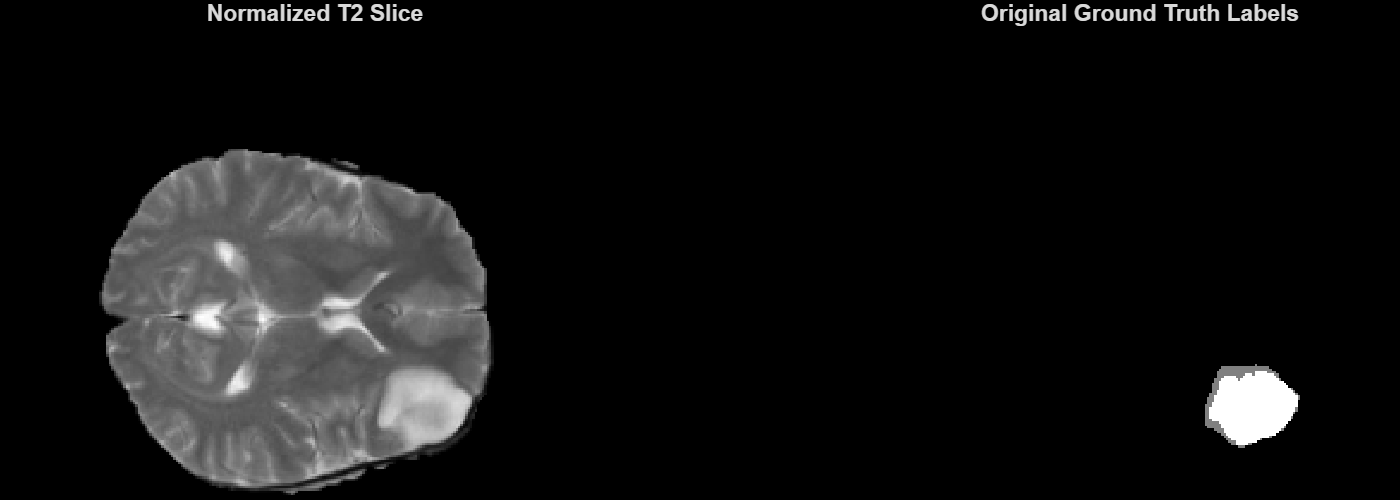
\includegraphics[width=0.9\linewidth]{images/baseline/best_case/01_data_understanding.png}
        \caption[Baseline Input]{Baseline Input: normalized T2 slice and expert-annotated ground truth}
        \label{fig:baseline_input}
    \end{subfigure}
    \vspace{0.1cm} % Spazio ridotto per evitare l'overflow verticale
    \begin{subfigure}[b]{\columnwidth}
        \centering
        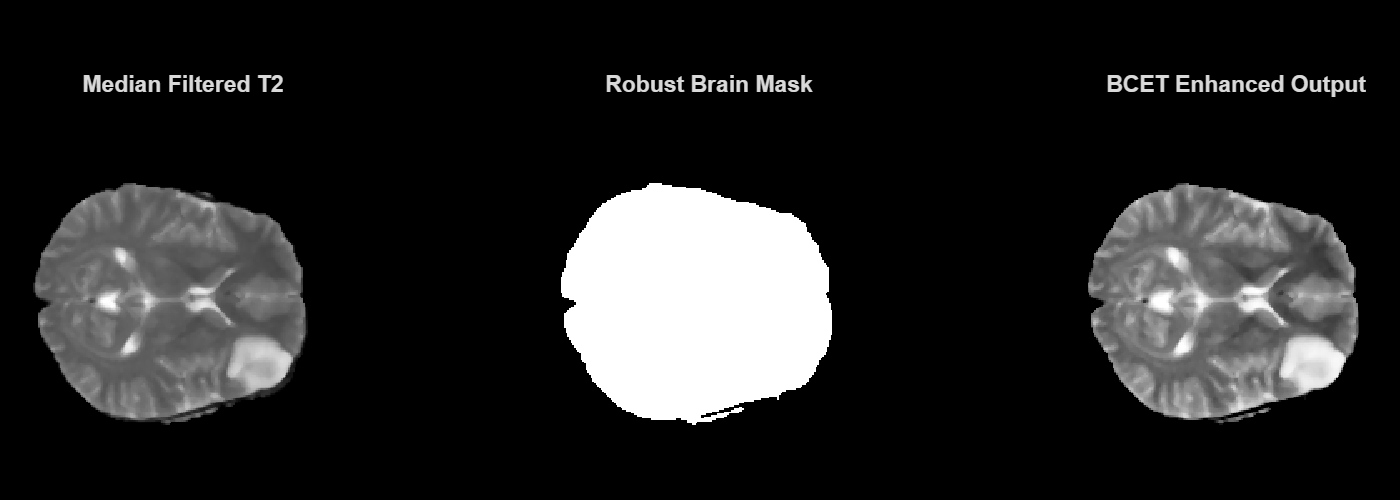
\includegraphics[width=0.9\linewidth]{images/baseline/best_case/02_enhancement.png}
        \caption[Pre-processing]{Pre-processing: median filter, Otsu brain mask, BCET enhancement}
        \label{fig:baseline_preprocessing}
    \end{subfigure}
    \vspace{0.1cm}
    \begin{subfigure}[b]{\columnwidth}
        \centering
        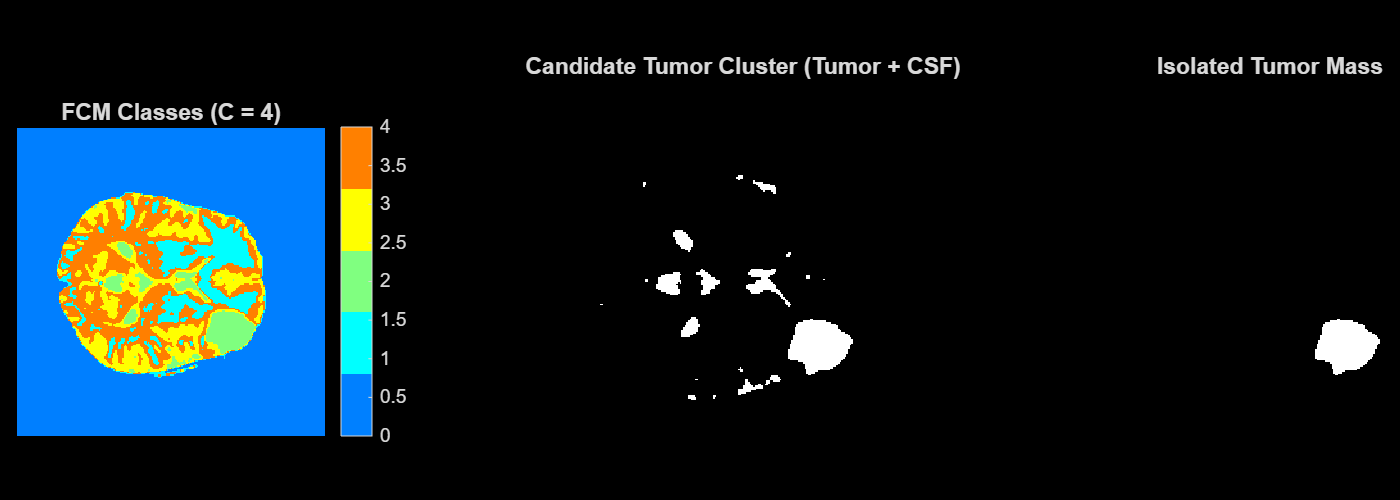
\includegraphics[width=0.9\linewidth]{images/baseline/best_case/03_segmentation.png}
        \caption{Four-class FCM segmentation and tumor-candidate isolation}
        \label{fig:baseline_segmentation}
    \end{subfigure}
    \vspace{0.1cm}
    \begin{subfigure}[b]{\columnwidth}
        \centering
        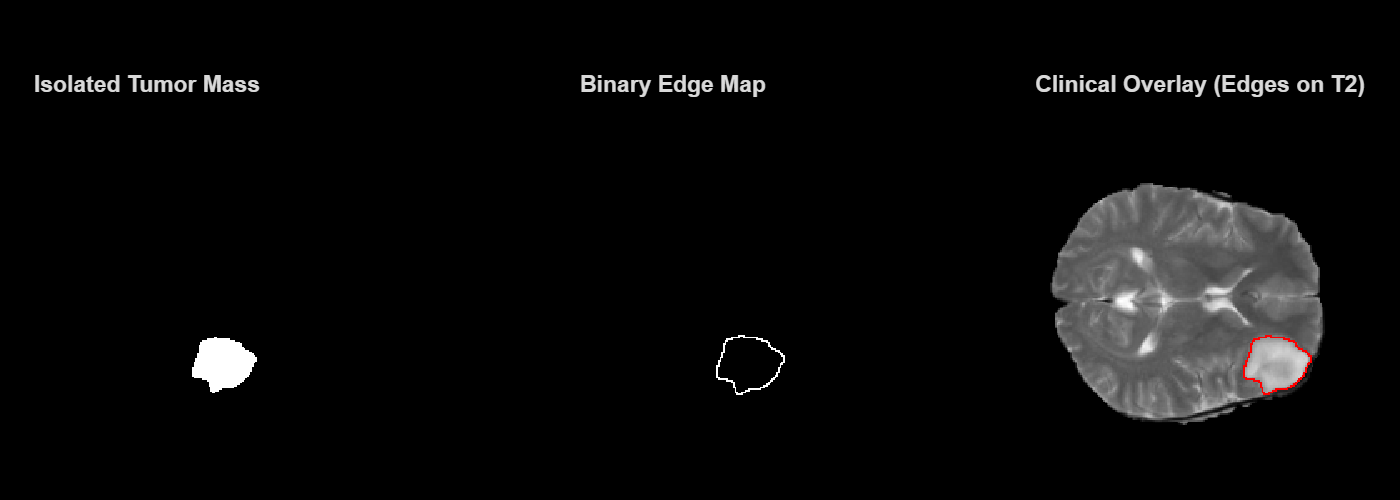
\includegraphics[width=0.9\linewidth]{images/baseline/best_case/04_edge_detection.png}
        \caption{Morphological edge extraction and clinical overlay}
        \label{fig:baseline_edge_extraction}
    \end{subfigure}
    \vspace{0.1cm}
    \begin{subfigure}[b]{\columnwidth}
        \centering
        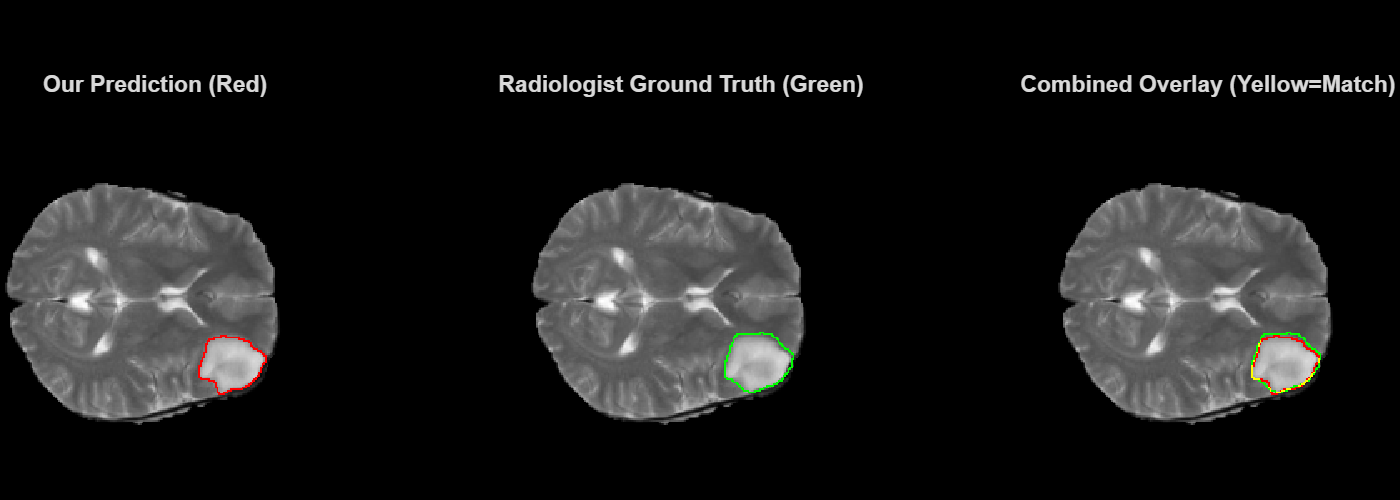
\includegraphics[width=0.9\linewidth]{images/baseline/best_case/05_final_validation.png}
        \caption{Validation: predicted boundary vs. expert ground truth}
        \label{fig:baseline_validation}
    \end{subfigure}
    \caption{End-to-end baseline on patient BRATS\_025 (best \gls{fom} case)}
    \label{fig:baseline_pipeline}
\end{figure}
 Because glioblastomas often outgrow their own blood supply, their core frequently becomes necrotic and hypointense rather than hyperintense, which can split the bright tumor candidate into a ring with a dark hole rather than a solid disc; the largest connected component is therefore hole-filled before isolation, so that the subsequent edge extraction traces only the outer boundary of the whole tumor, matching the convention used by the expert annotation. Finally, because the isolated tumor mask is already binary, a classical Canny detector would degenerate to simple perimeter tracing; a morphological edge detector (dilation of the mask minus the mask itself) is used instead, and applied identically to the reference mask, so that predicted and ground-truth boundaries are extracted with the same operator.\\
 Figure \ref{fig:validation_results} shows the comparison between three different cases: 
\begin{itemize}
    \item \textbf{best case}:the patient with the absolute highest FOM.
    \item \textbf{median case}:the patient whose FOM is as close as possible to the statistical median of all 484 values.
    \item \textbf{worst case}: the patient with the lowest FOM.
\end{itemize}
the predicted edges are in red, the expert ground truth is in green, and their combined overlay is yellow if both spatially match. The comparison is being made for the best, the median, and the worst \gls{fom} cases over the 484 BRATS patients.
\begin{figure}[htbp]
    \centering
    \captionsetup[subfigure]{justification=centering} 
    \begin{subfigure}[b]{\columnwidth}
        \centering
        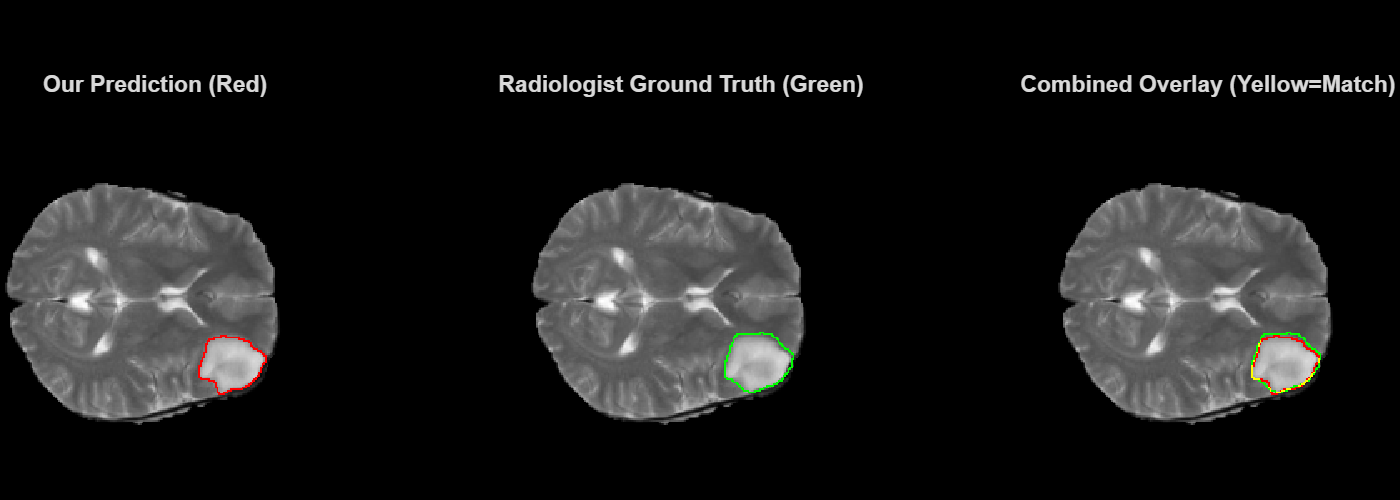
\includegraphics[width=0.9\linewidth]{images/baseline/best_case/05_final_validation.png}
        \caption{Best case: BRATS\_025 ($\mathrm{FOM}=0.847$)}
        \label{fig:baseline_best_cases}
    \end{subfigure}
    \vspace{0.1cm} 
    \begin{subfigure}[b]{\columnwidth}
        \centering
        
\includegraphics[width=0.9\linewidth]{images/baseline/median/05_final_validation.png}
        \caption{Median case: BRATS\_004 ($\mathrm{FOM}=0.136$)}
        \label{fig:baseline_median_cases}
    \end{subfigure}
    \vspace{0.1cm}
    \begin{subfigure}[b]{\columnwidth}
        \centering
        
\includegraphics[width=0.9\linewidth]{images/baseline/worst_case/05_final_validation.png}
        \caption{Worst case: BRATS\_012 ($\mathrm{FOM}=0.000$)}
        \label{fig:baseline_worst_cases}
    \end{subfigure}
    \caption{Baseline comparison between best case \ref{fig:baseline_best_cases}, median case \ref{fig:baseline_median_cases} and worst case \ref{fig:baseline_worst_cases}}
    \label{fig:validation_results}
\end{figure}
Accuracy stays uniformly high, mostly because boundary pixels are a tiny fraction of all pixels, but Sensitivity drops to a mean of just 10.7\%, far below the 85.8--97.4\% reported by Zotin et al. on their curated image pairs. Looking at the intermediate segmentation masks shows the main failure mode: on T2-weighted images, the brightest structures in the brain are very often the cerebrospinal fluid filling the ventricles, not the tumor. Even with the solidity-area check described above, the brightest-cluster heuristic often locks onto a compact, high-contrast \gls{csf} pocket instead of the more diffuse, lower-contrast tumor margin, so the extracted edges trace an anatomically correct but clinically irrelevant boundary. This problem does not show up on a small, manually curated test set, and only appears at the scale tested here; it motivates the optimized pipeline of Section \ref{sec:optimized}.
\begin{table}[htbp]
\centering
\caption{Baseline pipeline statistics over 484 BRATS patients.}
\label{tab:baseline_stats}
\begin{tabular}{lcc}
\toprule
Metric & Mean $\pm$ Std & Median \\
\midrule
Sensitivity (Pcd) & $0.107 \pm 0.088$ & $0.086$ \\
\gls{fom} & $0.193 \pm 0.186$ & $0.136$ \\
Accuracy & $0.974 \pm 0.014$ & $0.976$ \\
Pfa & --- & $3.877$ \\
\bottomrule
\end{tabular}
\end{table}
Table \ref{tab:baseline_stats} summarizes the results over the full dataset. The best, median, and worst cases by \gls{fom} are patients BRATS\_025 ($\mathrm{FOM}=0.847$), BRATS\_004 ($\mathrm{FOM}=0.136$), and BRATS\_012 ($\mathrm{FOM}=0.000$), respectively Fig. \ref{fig:baseline_best_cases}, Fig. \ref{fig:baseline_median_cases} and Fig. \ref{fig:baseline_worst_cases}. For 39 patients (8.1\%), the fixed central slice contains no ground-truth tumor voxels at all, making $\mathrm{Pcd}$ and $\mathrm{Pnd}$ undefined ($\mathrm{RECnt}=0$); these patients are excluded from the Sensitivity statistics but still contribute an $\mathrm{FOM}$ of zero, since a non-empty prediction with no reference edges yields no possible match. The pipeline did not raise an unhandled exception on any of the 484 patients, which suggests the brain-masking and cluster-selection steps are reasonably robust.
\section{Proposed Optimized Pipeline}\label{sec:optimized}
The validation in Section \ref{sec:baseline} identified two structural causes of failure that are independent of any single processing step: a static, content-agnostic slice selection that frequently misses the lesion altogether, and a T2-based hyperintensity criterion that cannot distinguish the tumor from \gls{csf}. The optimized pipeline addresses both causes directly, while reusing the median filtering, \gls{bcet} enhancement, and \gls{fcm} clustering stages of Section \ref{sec:baseline} unchanged.
The proposed optimizations were implemented in order to correct and overcome the two main structural causes:
\begin{itemize}
    \item \textbf{Dynamic slice selection.} Instead of the fixed central slice, the optimal axial slice is determined automatically from the full volume. A single hyperintensity threshold is computed as the 95th percentile of all intracranial voxel intensities in the volume, and the slice containing the largest number of voxels above this threshold is selected. The score is computed entirely from image intensities and never looks at the ground-truth mask, since a real, unlabeled scan would not provide one; an earlier version of this criterion selected the slice with the most ground-truth tumor pixels instead, which is label leakage and was corrected. As a proxy for "the slice most likely to contain the lesion" this criterion is imperfect but unsupervised, and it already reduces the number of patients whose selected slice contains no tumor at all from 39 (8.1\%, Section \ref{sec:baseline}) to 28 (5.8\%).
    \item \textbf{Multimodal transition to \gls{flair}.} The pipeline switches from the T2 to the \gls{flair} channel. \gls{flair} is a T2-weighted inversion-recovery sequence \cite{hajnal1992flair} whose preparation pulse is tuned to null the longitudinal magnetization of free water, physically suppressing the \gls{csf} signal that was identified in Section \ref{sec:baseline} as the dominant confound of the brightest-cluster heuristic. By removing the competing hyperintense structure at the acquisition level, the same intensity-based clustering and cluster-selection logic of the baseline can operate with substantially reduced ambiguity, without requiring any additional topological filter.
    \item \textbf{Dilated ground-truth evaluation.} Manual tumor tracing by a human expert carries an inherent sub-pixel positional uncertainty, and the morphological edge detector of Section \ref{sec:baseline} produces boundaries that are strictly one pixel wide, so that a clinically acceptable prediction offset by a single pixel would otherwise be scored as a complete miss. A tolerance band is therefore introduced by dilating the strict reference boundary with a disk of radius one pixel; $\mathrm{TP}$ is counted whenever a predicted edge pixel falls inside this band, while $\mathrm{FN}$ is still computed against the strict (undilated) boundary, so that $\mathrm{Pnd}$ and Sensitivity reflect the fraction of true boundary actually recovered. \gls{fom}, which already incorporates a continuous distance penalty, is left unchanged and computed on the strict boundary for direct comparability with Section \ref{sec:baseline}.
	\item \textbf{3-D tumor reconstruction (exploratory).} The validated single-slice detection above can be extended into a full 3-D reconstruction of the tumor within the brain volume. A single volume-wide \gls{bcet} enhancement and \gls{fcm} fit ($C=4$) is computed once for the whole brain, rather than refitting per slice, so that cluster assignment is consistent throughout the volume; this volumetric fit is a separate clustering pass used only for the 3-D reconstruction described below, and does not replace or alter the per-slice \gls{fcm} clustering that produces the quantitative results reported in Table \ref{tab:optimized_stats} and Figs. \ref{fig:optimized_pipeline}--\ref{fig:optimized_validation_results}. The lesion is then grown slice-by-slice from the already-validated 2-D detection on the dynamically-selected slice, accepting at each step only the candidate-cluster components overlapping the previously accepted slice; growth stops when the candidate area collapses to a sliver of the seed, or jumps abruptly, signalling that the front has latched onto an unrelated bright structure (e.g. periventricular tissue) rather than continuing the lesion. Fig. \ref{fig:3d_reconstruction} shows the reconstructed brain shell and tumor mass for patient BRATS\_213. Voxel-wise Dice overlap against the 3-D expert ground-truth volumes was computed over all 484 patients: mean $0.315 \pm 0.383$, median $0.044$. The distribution is strongly bimodal: 51 patients (10.5\%) produce a Dice of zero, largely coinciding with cases where the dynamically-selected slice contains no annotated tumor (see Section \ref{sec:optimized}); among the remaining 433 patients, mean Dice reaches $0.352$ and 171 patients (35.3\%) achieve Dice $> 0.5$, including BRATS\_213 (Dice $= 0.63$) and BRATS\_266 (Dice $= 0.78$). The reconstructed volume is systematically larger than the reference on all patients, consistent with the same edema-inclusive over-segmentation already observed at slice level. The high variance mirrors the already-documented spread of the 2-D pipeline (\gls{fom} std $= 0.273$): reconstruction quality is fundamentally bounded by per-patient seed quality, and is presented here as a qualitative extension rather than a clinically validated volumetric segmentation.
	
	\begin{figure}[htbp]
		\centering
		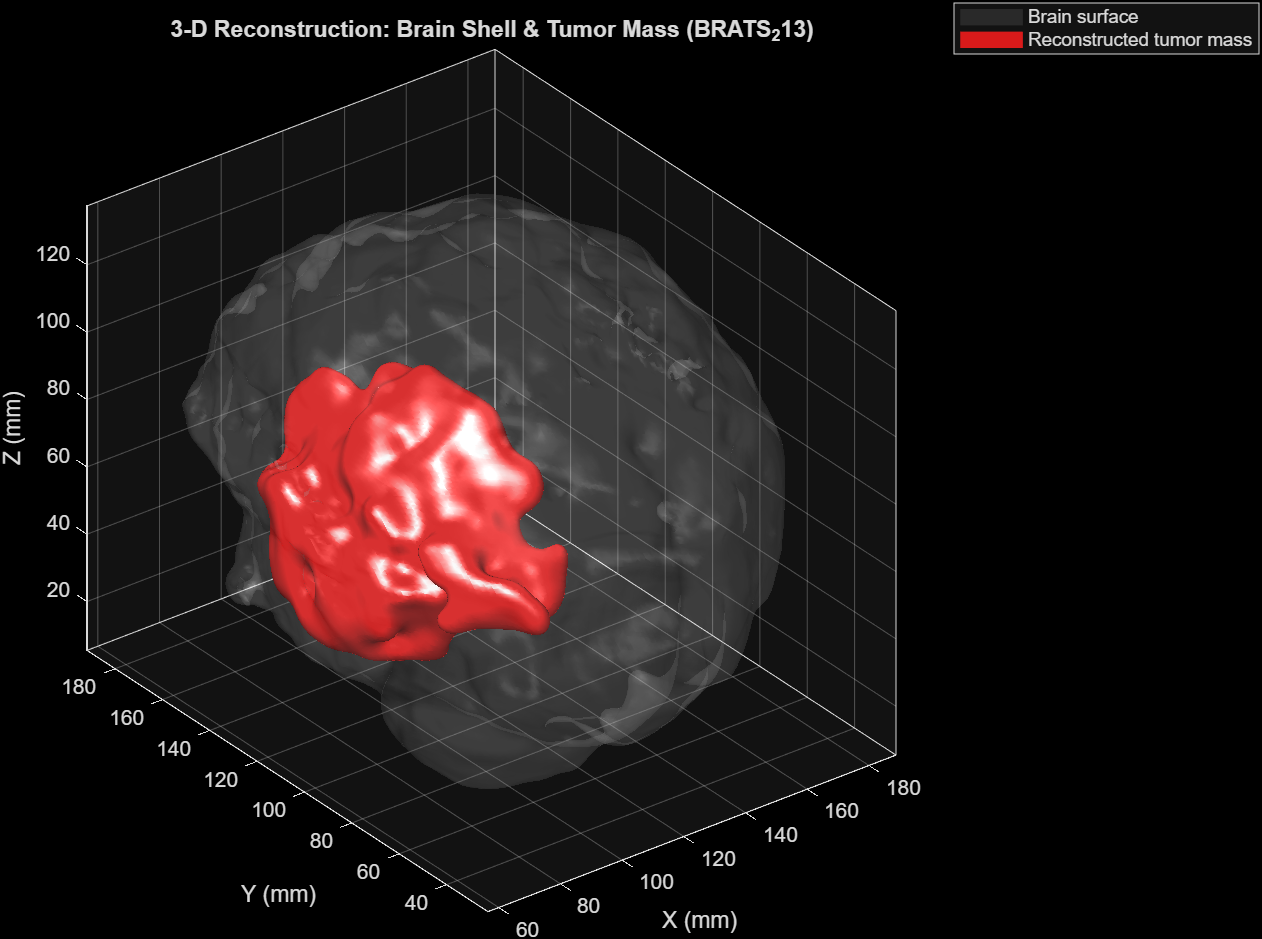
\includegraphics[width=0.9\columnwidth]{images/optimized/best_case/reconstruction.png}
		\caption{3-D reconstruction of patient BRATS\_213: brain surface (translucent gray) and reconstructed tumor mass (red), grown from the validated 2-D detection at the dynamically-selected slice.}
		\label{fig:3d_reconstruction}
	\end{figure}
	
\end{itemize}
Figure \ref{fig:optimized_pipeline} shows the same five stages applied to patient BRATS\_213, the best-\gls{fom} case of the optimized pipeline. The main difference between the optimized pipeline and the baseline is that Panel \ref{fig:optimized_input} shows the \gls{flair} slice selected by the dynamic slice-selection criterion, alongside its ground truth.
\begin{figure}[htbp]
    \captionsetup[subfigure]{justification=centering} 
    \begin{subfigure}[b]{\columnwidth}
        \centering
        
\includegraphics[width=0.9\linewidth]{images/optimized/best_case/01_data_understanding.png}
        \caption[Optimized Input]{normalized FLAIR slice (dynamically selected) and expert-annotated ground truth}
        \label{fig:optimized_input}
    \end{subfigure}
    \vspace{0.1cm}
    \begin{subfigure}[b]{\columnwidth}
        \centering
        
\includegraphics[width=0.9\linewidth]{images/optimized/best_case/02_enhancement.png}
        \caption[Pre-processing]{Pre-processing: median filter, Otsu brain mask, BCET enhancement}
        \label{fig:optimized_preprocessing}
    \end{subfigure}
    \vspace{0.1cm}
    \begin{subfigure}[b]{\columnwidth}
        \centering
        
\includegraphics[width=0.9\linewidth]{images/optimized/best_case/03_segmentation.png}
        \caption{Four-class FCM segmentation and tumor-candidate isolation}
        \label{fig:optimized_segmentation}
    \end{subfigure}
    \vspace{0.1cm}
    \begin{subfigure}[b]{\columnwidth}
        \centering
        
\includegraphics[width=0.9\linewidth]{images/optimized/best_case/04_edge_detection.png}
        \caption{Morphological edge extraction and clinical overlay}
        \label{fig:optimized_edge_extraction}
    \end{subfigure}
    \vspace{0.1cm}
    \begin{subfigure}[b]{\columnwidth}
        \centering
        
\includegraphics[width=0.9\linewidth]{images/optimized/best_case/05_final_validation.png}
        \caption{Validation: predicted boundary vs. expert ground truth}
        \label{fig:optimized_validation}
    \end{subfigure}
    \caption{End-to-end optimized pipeline on patient BRATS\_213 (best FOM case)}
    \label{fig:optimized_pipeline}
\end{figure}
Table \ref{tab:optimized_stats} reports the dataset-wide statistics.
\begin{table}[htbp]
\centering

\caption{Optimized pipeline statistics over 484 BRATS patients.}
\label{tab:optimized_stats}
\begin{tabular}{lcc}
\toprule
Metric & Mean $\pm$ Std & Median \\
\midrule
Sensitivity (Pcd) & $0.248 \pm 0.178$ & $0.241$ \\
\gls{fom} & $0.283 \pm 0.273$ & $0.171$ \\
Accuracy & $0.980 \pm 0.011$ & $0.981$ \\
Pfa & --- & $2.471$ \\
\bottomrule
\end{tabular}
\end{table}

The best, median, and worst cases by \gls{fom} are now patients BRATS\_213 ($\mathrm{FOM}=0.928$), BRATS\_266 ($\mathrm{FOM}=0.171$), and, notably, again BRATS\_012 ($\mathrm{FOM}=0.000$).For this patient, the \gls{flair} hyperintensity criterion selects a different axial slice (Z=43) than the fixed central slice used in the baseline, yet that slice also contains no ground-truth tumor voxels, so neither pipeline detects any reference boundary to compare against. 
\begin{figure}[htbp]
    \centering
    \captionsetup[subfigure]{justification=centering} 
    \begin{subfigure}[b]{\columnwidth}
        \centering
        
\includegraphics[width=0.9\linewidth]{images/optimized/best_case/05_final_validation.png}
        \caption{Best case: BRATS\_213 ($\mathrm{FOM}=0.928$)}
        \label{fig:optimized_best_cases}
    \end{subfigure}
    \vspace{0.1cm} 
    \begin{subfigure}[b]{\columnwidth}
        \centering
        
\includegraphics[width=0.9\linewidth]{images/optimized/median/05_final_validation.png}
        \caption{Median case: BRATS\_266 ($\mathrm{FOM}=0.171$)}
        \label{fig:optimized_median_cases}
    \end{subfigure}
    \vspace{0.1cm}
    \begin{subfigure}[b]{\columnwidth}
        \centering
        
\includegraphics[width=0.9\linewidth]{images/optimized/worst_case/05_final_validation.png}
        \caption{Worst case: BRATS\_012 ($\mathrm{FOM}=0.000$)}
        \label{fig:optimized_worst_cases}
    \end{subfigure}
    \caption{Optimized pipeline comparison between best case \ref{fig:optimized_best_cases}, median case \ref{fig:optimized_median_cases} and worst case \ref{fig:optimized_worst_cases}}
    \label{fig:optimized_validation_results}
\end{figure}
This recurring failure shows that, even though the proposed slice-selection proxy is more reliable on average, it is still a heuristic and gives no guarantee for atypical or very small lesions that do not stand out in the volume-wise hyperintensity statistics. The additional 3-D volume scan required by dynamic slice selection adds little overhead in practice, since computing a percentile and a per-slice voxel count over the volume is cheap compared to the rest of the pipeline: mean processing time per patient rises from 0.99 s for the baseline to 1.06 s for the optimized pipeline, an 8\% increase.

\section{Critical Discussion and Comparison}\label{sec:comparison}
Table \ref{tab:comparison} consolidates the dataset-wide results of Sections \ref{sec:baseline} and \ref{sec:optimized}. The optimized pipeline improves mean Sensitivity by 132\% (from 0.107 to 0.248) and mean \gls{fom} by 46\% (from 0.193 to 0.283), while mean Accuracy, already saturated by class imbalance, improves only marginally (from 0.974 to 0.980).

\begin{table}[htbp]
\centering
\caption{Baseline vs. optimized pipeline, mean values over 484 patients.}
\label{tab:comparison}
\begin{tabular}{lccc}
\toprule
Metric & Baseline & Optimized & Change \\
\midrule
Sensitivity (Pcd) & $0.107$ & $0.248$ & $+132\%$ \\
\gls{fom} & $0.193$ & $0.283$ & $+46\%$ \\
Accuracy & $0.974$ & $0.980$ & $+0.7\%$ \\
\bottomrule
\end{tabular}
\end{table}

These gains match the two causes found in Section \ref{sec:baseline}. Switching to \gls{flair} removes the \gls{csf} hyperintensity that competed with the tumor for the brightest \gls{fcm} cluster, and dynamic slice selection reduces, without eliminating, the fraction of patients whose processed slice contains no tumor at all, from 8.1\% to 5.8\%. Both changes act on the input to the pipeline, not on the clustering or edge-extraction logic. This suggests that the original bottleneck was mainly about the input given to the pipeline -- the contrast mechanism and the slice chosen -- rather than the segmentation algorithm itself.

Accuracy stays above 0.97 in both pipelines even when baseline Sensitivity is as low as 11\%. This is a known limitation of pixel-wise accuracy on heavily imbalanced segmentation tasks: boundary pixels are a small fraction of the image, so a prediction that almost completely misses the tumor is still "correct" on most background pixels. This is why Sensitivity and \gls{fom}, not Accuracy, are the metrics that matter for clinical reliability, and why the baseline pipeline can look visually reasonable in Section \ref{sec:baseline} while still being clinically unusable.

The two pipelines also share a blind spot. The same worst-case patient identified in Sections \ref{sec:baseline} and \ref{sec:optimized} gets $\mathrm{FOM}=0$ under both the fixed central slice and the \gls{flair}-hyperintensity criterion, because neither heuristic lands on an axial slice that intersects the annotated lesion. This shows that dynamic slice selection, although more robust on average, is still a 2-D, volume-statistics-based proxy and not an explicit localization of the tumor; it gives no guarantee for small or eccentrically located lesions that do not stand out in the global hyperintensity histogram. The \gls{fcm} cluster-selection heuristic of Section \ref{sec:baseline} has a similar limitation: even with the 40\% area cap and the solidity-area score, it is still an intensity-and-shape-only criterion with no spatial or anatomical prior. The multimodal contrast change, not a change to this heuristic, is responsible for most of the measured improvement. Finally, the dilated evaluation metric of Section \ref{sec:optimized} makes Sensitivity easier to interpret clinically, but by construction it is more permissive than the strict metric of Section \ref{sec:baseline}. The \gls{fom}, computed identically on strict boundaries in both pipelines, is therefore the more conservative and directly comparable indicator of the 46\% improvement reported above. The optimized pipeline reaches these results at a similar computational cost (Section \ref{sec:optimized}), which matters given its intended use on large-scale clinical datasets.
\section{Conclusions}\label{sec:conclusions}
This work reproduced the unsupervised edge detection pipeline of Zotin et al. \cite{zotin2018edge} and validated it on 484 multiparametric volumes from the \gls{msd} Brain Tumor task \cite{antonelli2022medical}, a scale two orders of magnitude larger than the 30 hand-picked images used in the original study. This large-scale validation revealed a weakness that a small curated dataset does not show: mean Sensitivity dropped to 10.7\%, mainly because of confusion between tumor and \gls{csf} hyperintensity on T2-weighted images, and because a static central-slice selection did not even intersect the annotated lesion for 8.1\% of patients. The proposed optimized pipeline addressed both causes at the input level, without modifying the underlying \gls{fcm} clustering or edge-extraction logic, by combining an unsupervised dynamic slice search with a multimodal transition to \gls{flair} sequences and a spatially tolerant evaluation metric. This yielded a 132\% increase in mean Sensitivity and a 46\% increase in mean \gls{fom}, at a small additional computational cost. Overall, this suggests that the reliability of an otherwise unchanged unsupervised, intensity-based segmentation method depends as much on the physical contrast mechanism and the spatial cross-section it is given as on the clustering algorithm itself: changing the input modality and the slice-selection criterion recovered most of the performance gap, while the clustering and edge-extraction stages stayed the same. At the same time, the shared zero-\gls{fom} failure on the same patient across both pipelines shows that a global, volume-statistics-based proxy for tumor localization, however effective on average, is not a substitute for an explicit spatial or shape prior, and can still fail outright on small or eccentrically located lesions. Future work should target this remaining gap directly, for instance through deterministic or atlas-based centroid initialization for \gls{fcm} \cite{benson2016brain, szilagyi2003mri}, morphological skull-stripping refinements to further constrain the clustering search space \cite{hooda2014brain}, a purely spatial criterion that discounts centrally-located clusters under the prior that the lateral ventricles, unlike most tumors, sit near the brain's geometric center -- a lower-cost alternative to the \gls{flair} transition when only T2 is available -- or a learned, supervised localization step to replace the unsupervised hyperintensity proxy for slice and region selection. More generally, this study suggests that unsupervised medical segmentation pipelines should be evaluated, whenever feasible, on large and heterogeneous clinical datasets rather than on small curated samples, since the latter can hide failure modes that only show up at scale. More broadly, the entire pipeline studied here belongs to a class of unsupervised, intensity-based methods that has been substantially superseded in the medical imaging literature by supervised deep learning \cite{magadza2021survey}. Architectures such as U-Net \cite{ronneberger2015unet} and its self-configuring descendant nnU-Net \cite{isensee2021nnunet} learn, directly from labeled examples, hierarchical spatial features that jointly encode intensity, shape, and anatomical context -- precisely the spatial and anatomical prior that this study found missing from both the \gls{fcm} cluster-selection heuristic and the volume-statistics-based slice selection. Trained end-to-end on datasets such as the \gls{msd} Brain Tumor task used here \cite{antonelli2022medical}, these models require no hand-tuned brain mask, no fixed number of clusters, and no brightness-based rule to disambiguate the tumor from \gls{csf}: the segmentation boundary is learned jointly with the features that define it. As a concrete reference point, an nnU-Net variant placed first in the BraTS 2020 challenge with Dice scores of 0.890, 0.851, and 0.820 for whole tumor, tumor core, and enhancing tumor respectively \cite{isensee2020brats} -- figures well beyond what intensity-only clustering can reach on the same task. The corresponding cost is that these methods require a labeled training set and non-trivial training-time compute, whereas the pipeline studied here needs no training data at all and remains fully interpretable at every stage -- which keeps it relevant as a fast, equipment-agnostic baseline, an annotation-assisting tool, or a teaching example of classical image processing -- but for raw segmentation and edge-detection accuracy on annotated clinical datasets, deep learning is, at this point, the dominant and recommended approach.

\bibliographystyle{IEEEtran} 
\bibliography{biblios}
\end{document}